%TEX root = ../dissertation.tex

\chapter{Methods}
\label{chapter:Uncertainty_Estimation}

This chapter outlines the methodological framework used in this thesis to estimate and evaluate MOSA's uncertainty. It starts by explaining how uncertainty can be extracted from the model's latent space and how the sampled latent representations can be propagated through the decoder to obtain predictive distributions for the reconstructed datasets. It then introduces Monte Carlo Dropout as a complementary uncertainty estimation method, followed by the sharpness, calibration and proper scoring metrics used to evaluate the resulting predictive distributions.
 
\section{Latent Space Extraction and Sampling} \label{Latent_Space_Sampling}

As previously mentioned, the variational autoencoder architecture is composed of an encoder, a probabilistic latent space and a decoder. The probabilistic latent space used in \citep{Cai2024} follows a learned multivariate Gaussian distribution, sampled during training. This sampling enables gradient-based optimisation through the stochastic latent space via the reparametrisation trick and also  enforces a smooth representation to help the reconstruction of new data. During the prediction, the model uses the mean of this learned Gaussian distribution as the values of the latent space. This multivariate Gaussian latent space also provides methods for estimating the model's uncertainty not present in other deep learning model architectures.

The variational nature of the model allows us to characterise uncertainty in two complementary ways. The first way is by extracting the mean and variance matrices of the joint latent space, as illustrated in Figure \ref{fig:encoder_and_var_extracted}. The model's encoder outputs two tensors, corresponding to the mean and the logarithmic variance of the joint latent space's multivariate Gaussian distribution. These matrices provide information on the variability of the latent dimensions, represented by their columns, and of the cell lines used as training data, represented by their rows.

These two matrices provide a direct way to quantify the encoder's uncertainty about the inferred latent representation for each sample, that is, how confidently the encoder maps an input into latent space. The variance matrix indicates how much the latent representation is expected to spread around its mean. A higher variance value corresponds to lower confidence in that particular latent code, while lower variance corresponds to a more concentrated belief around the mean. This uncertainty primarily reflects ambiguity in the data and in the learned representation, not uncertainty over the encoder's parameters themselves, which remain fixed after training. Using the reparametrisation trick, we may also sample from the latent space, which enables data visualisation methods such as \gls{UMAP}, a widely used approach for visualising high-dimensional biological data.

\begin{figure}[!ht]
    \centering
    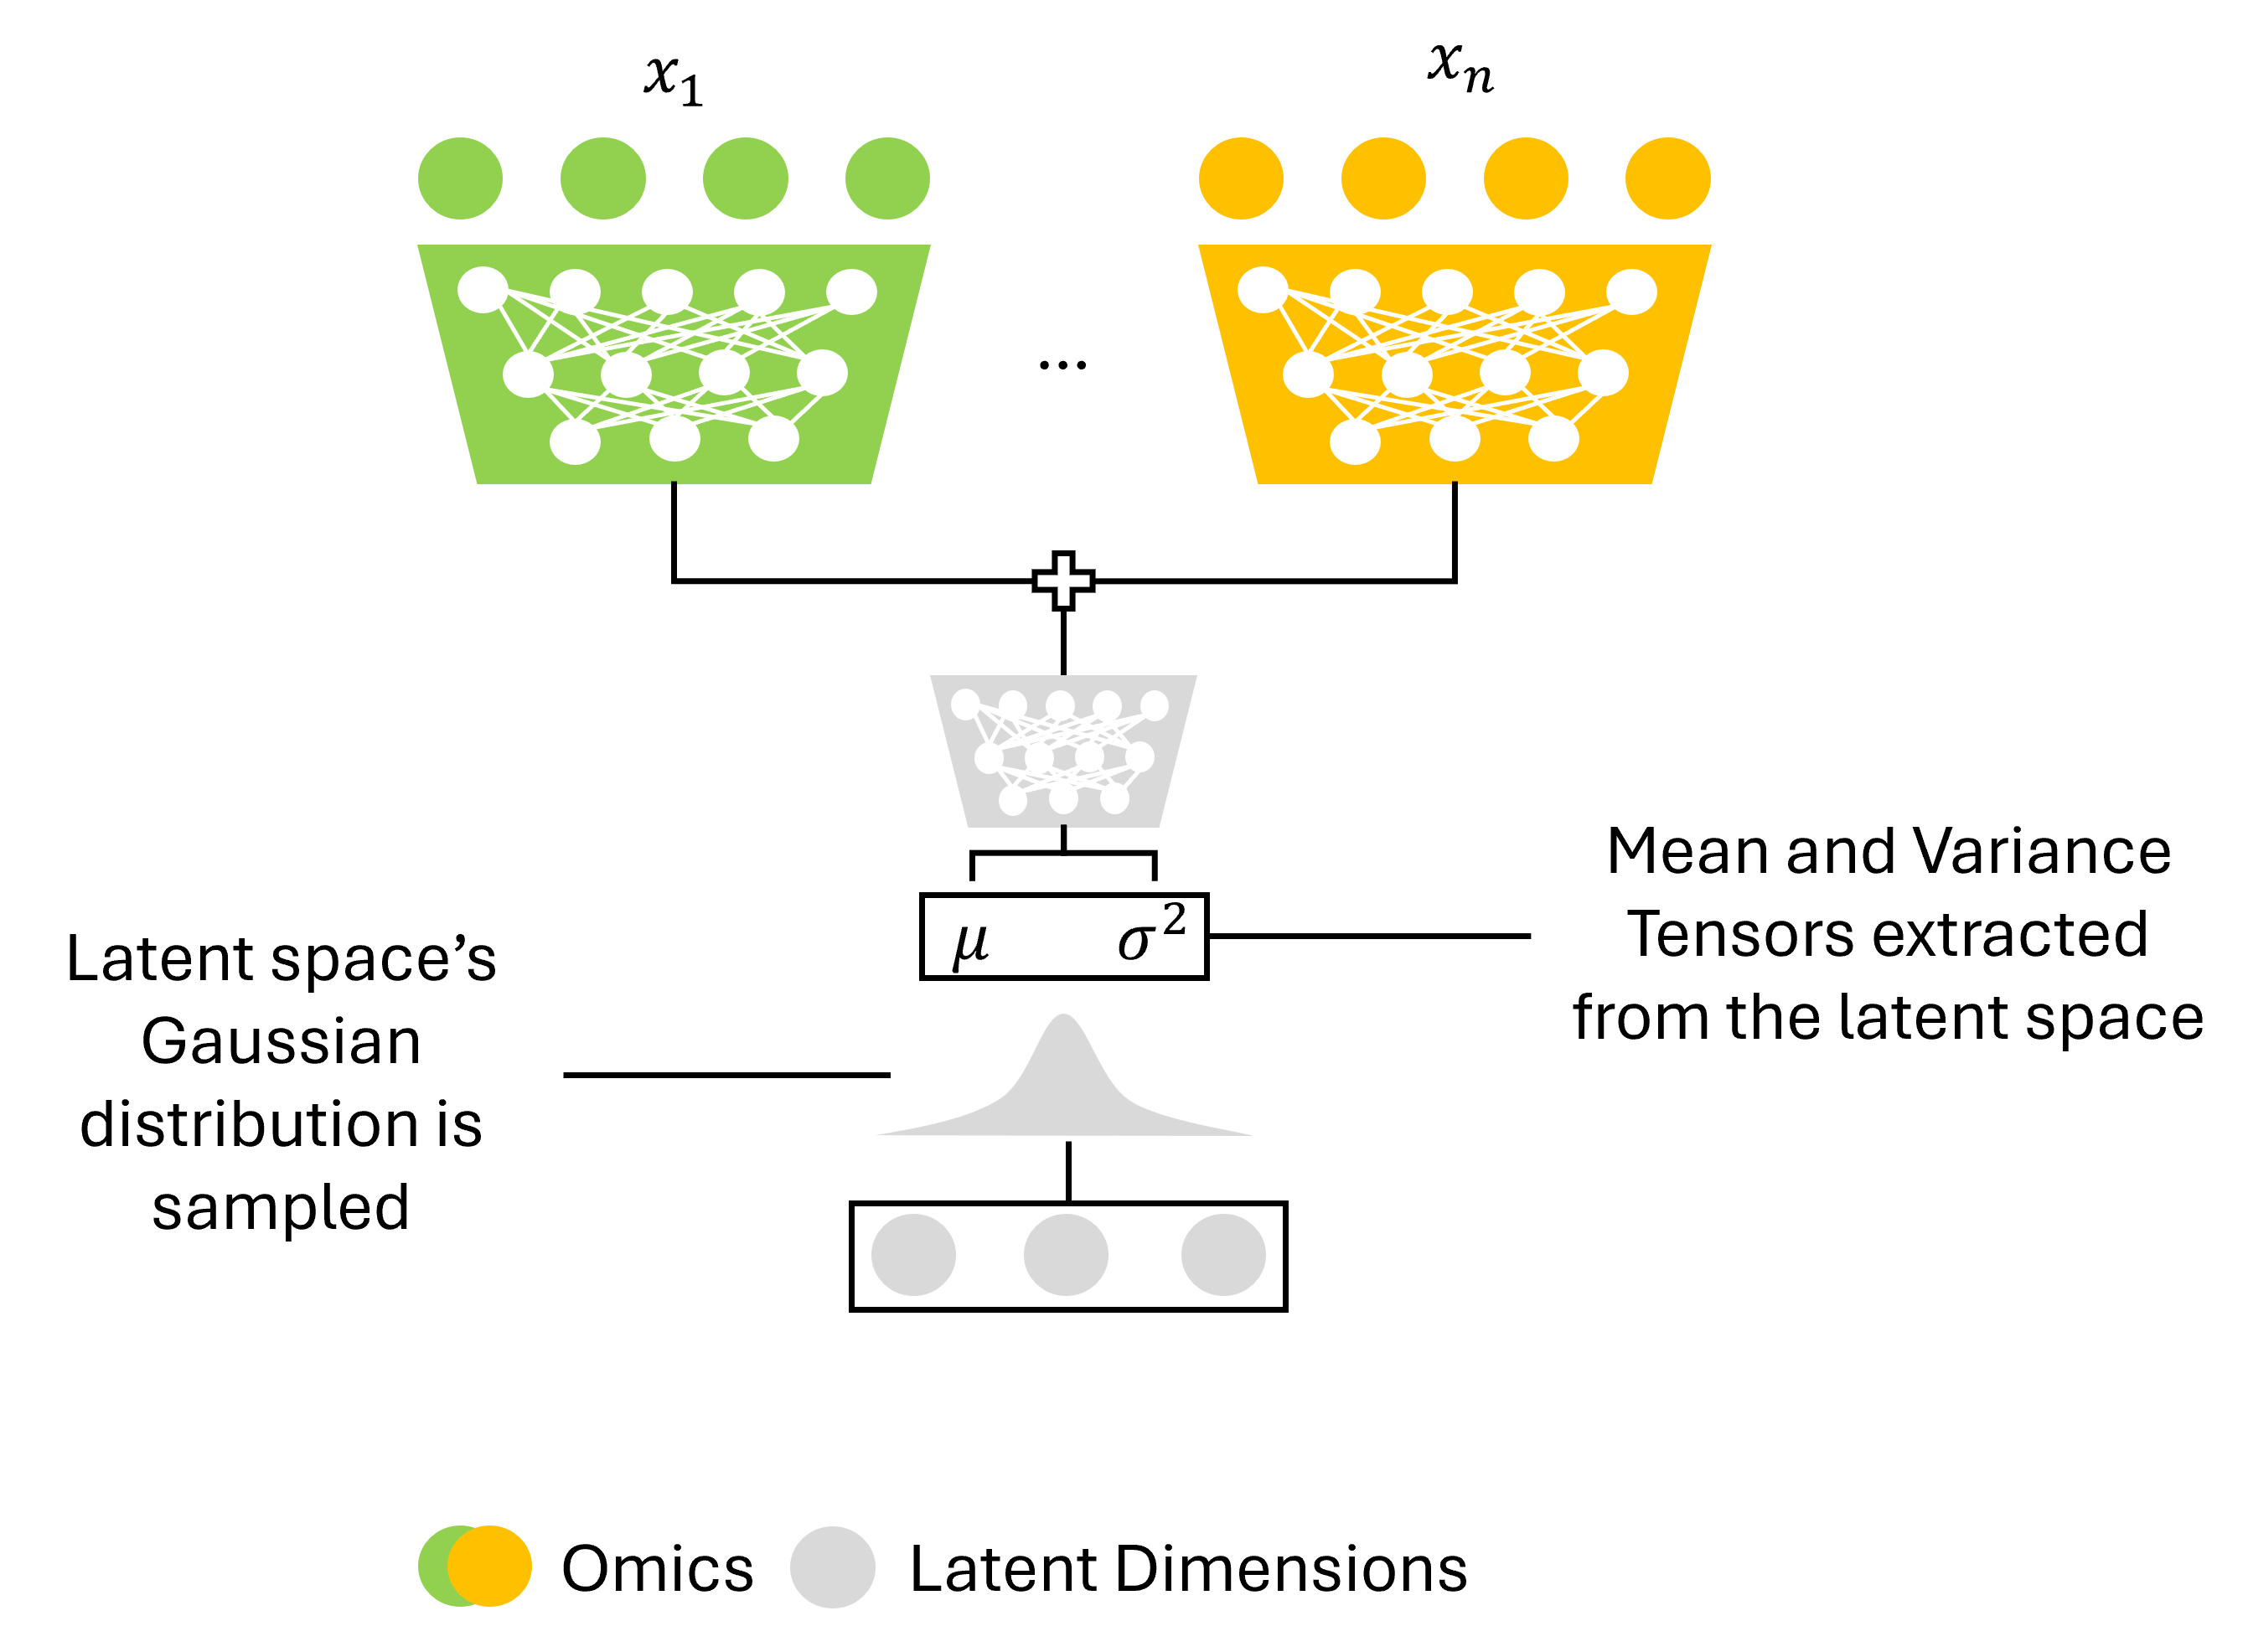
\includegraphics[width=0.5\linewidth]{images/Mosa_sample_encoder.png}
    \caption[Schematic of the Latent Space Sampling method]{Schematic of the model's, \gls{MOSA}'s, autoencoder and latent space with indication of where the Mean and Variance tensors are extracted along with where the latent space is sampled.}
    \label{fig:encoder_and_var_extracted}
\end{figure}

We may also take these samples of the latent space and pass them through the model's decoder, as illustrated in Figure \ref{fig:sample_decoder}. This allows us to obtain samples of the model's output across the seven omics. From these samples we can approximate, for each data point, the predictive distribution implied by the latent variable and decoder, thus providing a basis to compute sharpness and calibration metrics as well as proper scoring rules to evaluate predictive uncertainty. These quantities provide insight primarily into the decoder's aleatoric uncertainty captured by the generative model.

The output of this sampling method is seven three-dimensional matrices. The dataset number corresponds to the seven omics under study. The three dimensions, ($x$, $y$, $z$), correspond to the predicted cell lines, features and the $n$ samples. For this thesis the value of $n$ for the samples was set at 100. A larger number of samples leads to more accurate estimation of the model's true uncertainty but it leads to a more computationally intensive analysis; 100 samples were chosen as a trade-off between statistical reliability and computational costs.

\begin{figure}[!ht]
    \centering
    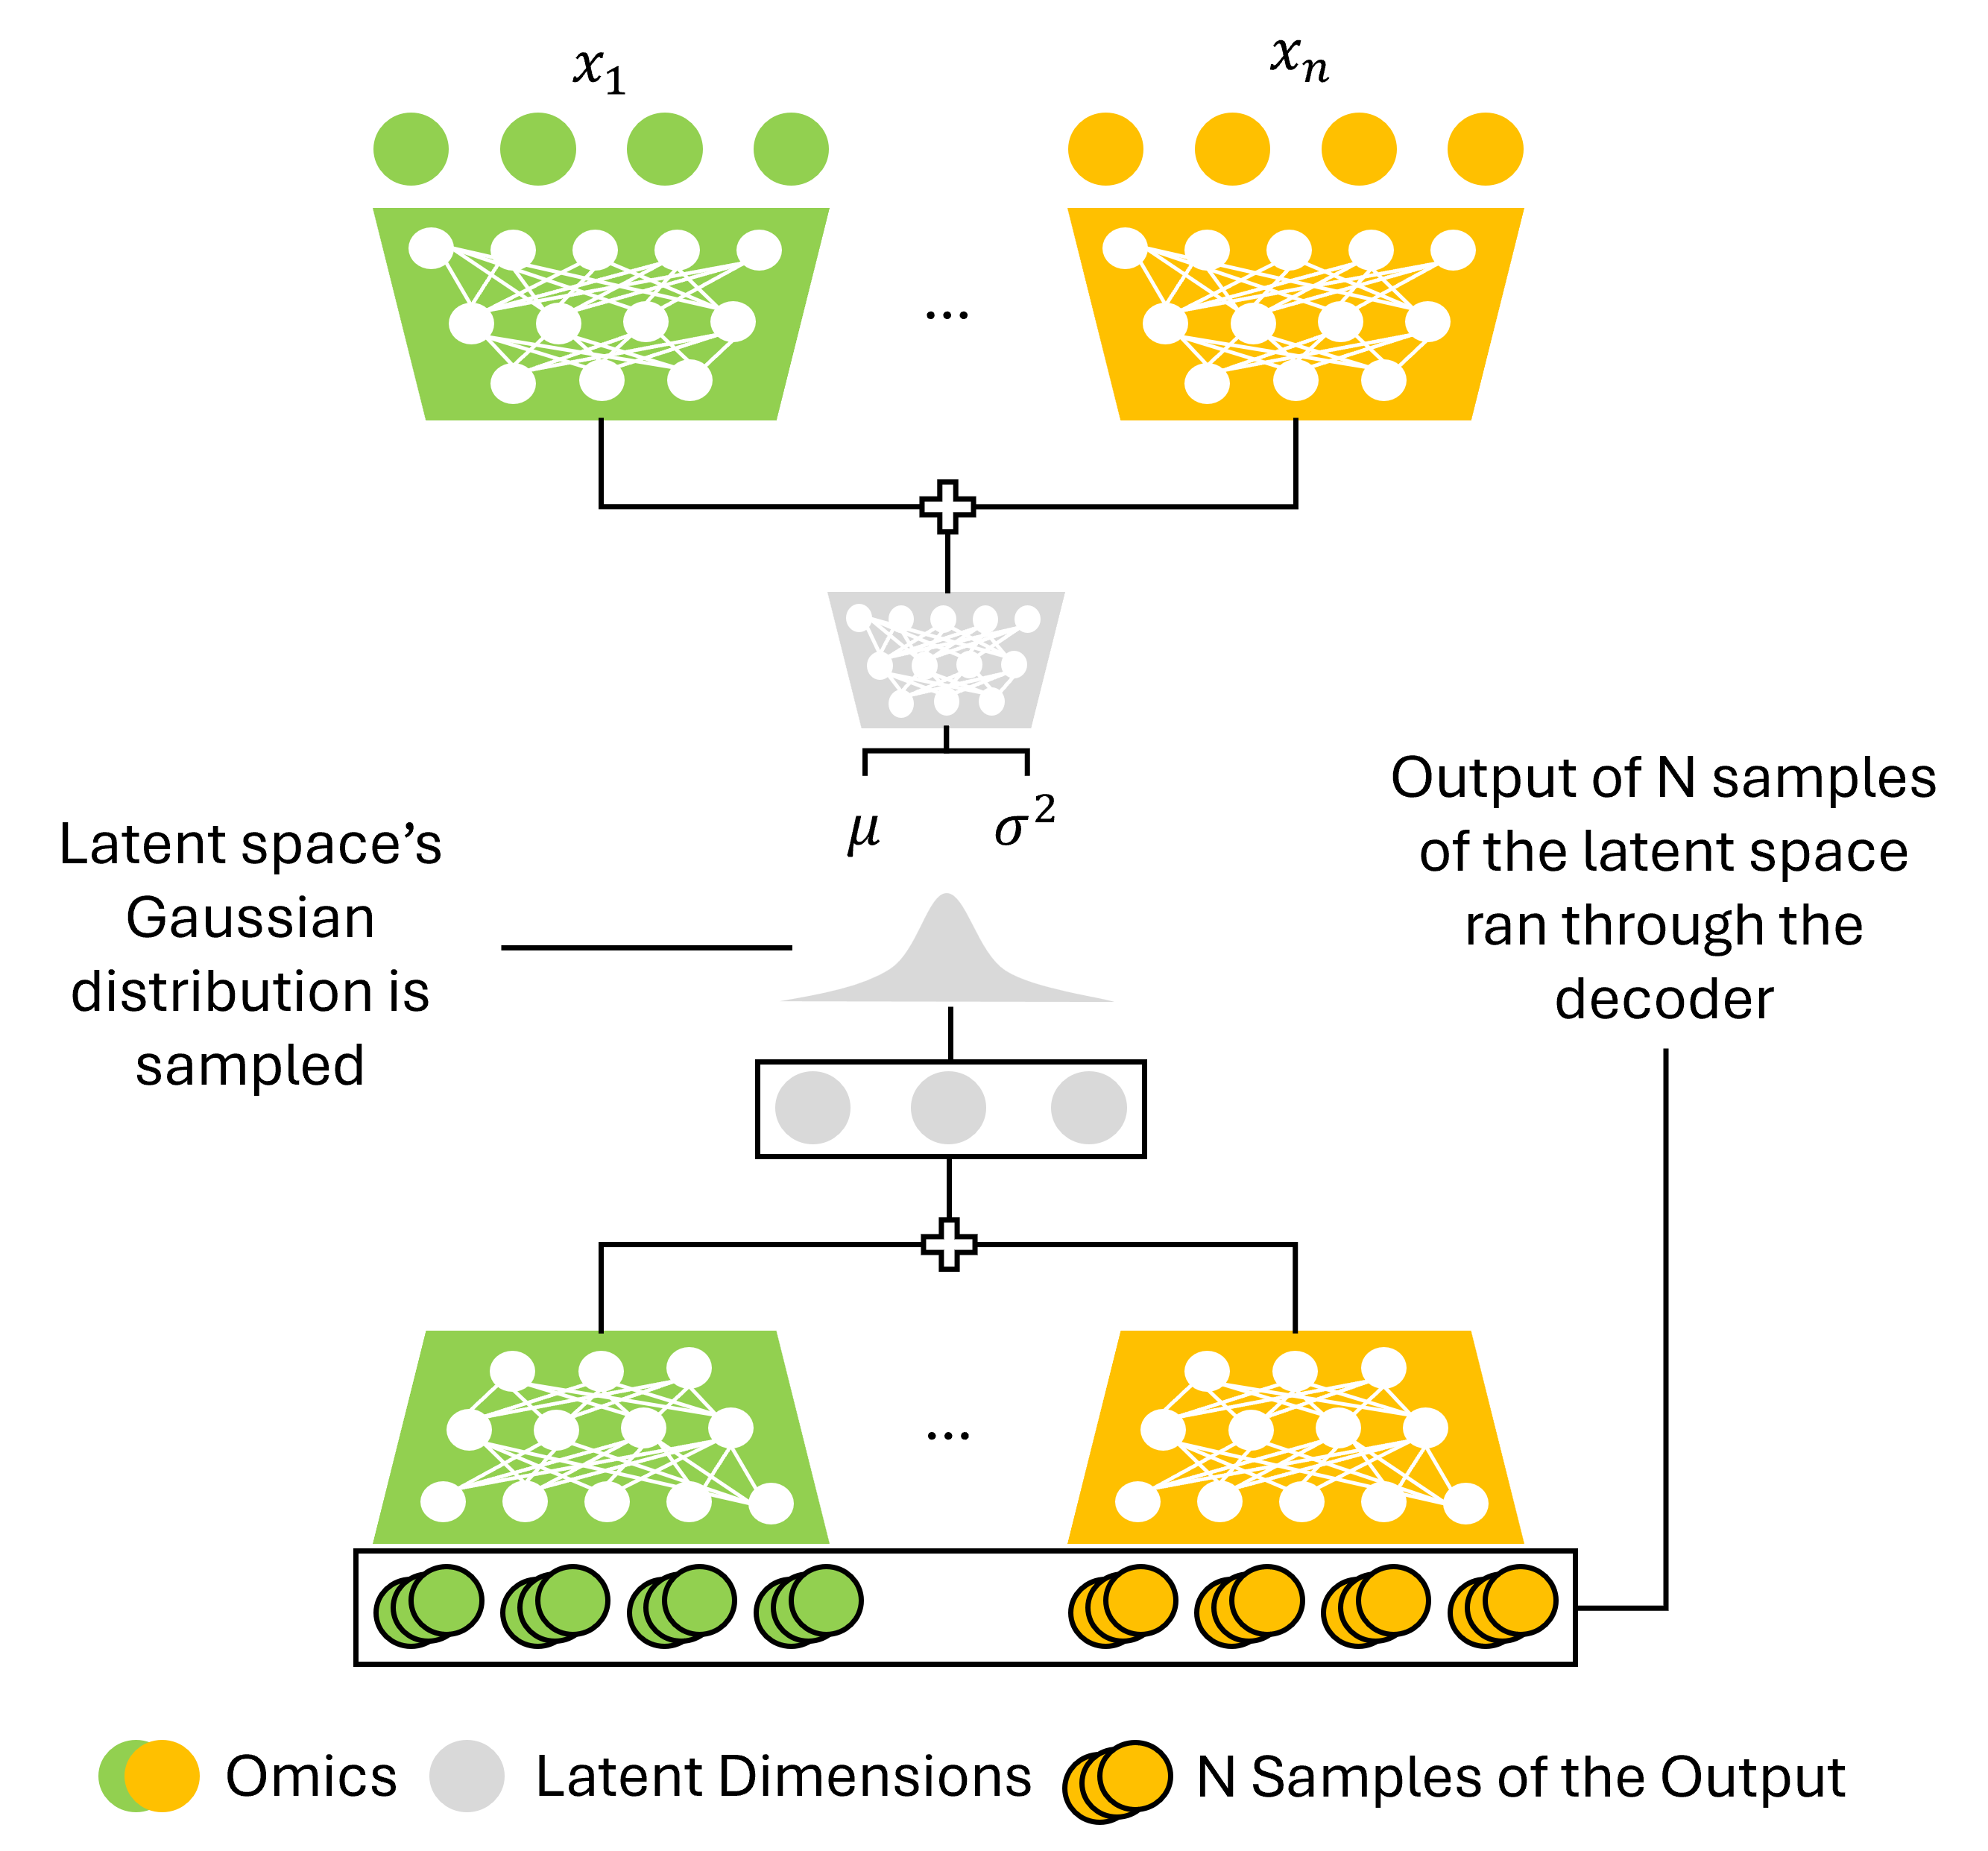
\includegraphics[width=0.5\linewidth]{images/Mosa_sample_full.png}
    \caption[Schematic of Latent Space Sampling run through MOSA's decoder]{Schematic of the autoencoder, \gls{MOSA}, and the sample method of the joint latent space run through the model's decoder.}
    \label{fig:sample_decoder}
\end{figure}


\section{Monte Carlo Dropout} \label{Monte_Carlo_Dropout}


\Gls{MCD} has established itself as a prominent and widely used approximation to Bayesian inference in deep learning, offering a practical mechanism for estimating predictive uncertainty with only minimal changes to standard architectures and training procedures \citep{Gal2016Dropout}.

Originally, dropout was proposed as a stochastic regularisation technique to reduce overfitting in neural networks by randomly setting a subset of hidden neurons to zero during training. This helps prevent dependency between features and reduces overfitting, improving generalisation performance \citep{Srivastava2014Dropout}. From this perspective, dropout can be understood as implicitly training multiple subnetworks that share the same parameters, with a form of model averaging occurring at test time when the full network is used with rescaled weights \citep{Srivastava2014Dropout}. Gal and Ghahramani \citep{Gal2016Dropout}, however, provided a Bayesian interpretation of dropout, demonstrating that a neural network with dropout applied before every weight layer is mathematically equivalent to performing approximate variational inference in a deep Gaussian process. Under this interpretation, the random binary masks induced by dropout correspond to samples from a variational distribution over the network weights.

This theoretical perspective leads directly to the Monte Carlo Dropout procedure for uncertainty estimation. Given an input $x$ and a trained neural network $f(\cdot; \theta)$ with dropout layers, the approximate predictive distribution is obtained by performing multiple stochastic forward passes with dropout active at inference time, rather than disabled as in standard practice \citep{Gal2016Dropout}. At each pass $t$, a dropout mask $M_t$ is sampled from a Bernoulli distribution with parameter $p$, giving rise to an effective parameter realisation $\theta_t = M_t \odot \theta$, where $\odot$ denotes element-wise multiplication. Repeating this process $T$ times yields a collection of stochastic predictions $\{ f(x; \theta_t) \}_{t=1}^T$, from which the predictive mean and variance can be estimated as Monte Carlo moments. The sample mean serves as an approximation of the Bayesian model average prediction, while the sample variance reflects the spread of predictions across different dropout-induced subnetworks and provides an estimate of the model's epistemic uncertainty \citep{Gal2016Dropout}.

In a generative model such as the VAE considered in this thesis, MCD can be integrated into both the encoder and decoder components without altering the latent variable formulation introduced earlier. While \gls{MOSA} has three different forms of dropout integrated, the commonly used neuron dropout, feature-wise dropout and view-wise dropout, only neuron-wise dropout will be considered for Monte Carlo Dropout.

Applying dropout to the encoder network leads to a distribution over approximate posterior parameters for the latent variables, and repeated stochastic forward passes allow the characterisation of uncertainty in the inferred latent representation of each input. Similarly, applying dropout to the decoder network enables the estimation of uncertainty in the reconstructed data or generated samples conditioned on a latent code. In both cases, the use of Monte Carlo sampling at inference time transforms deterministic VAE outputs into distributions that encode information about model confidence.

In this thesis, Monte Carlo Dropout is applied only to MOSA's decoder. The encoder is used deterministically and the mean of the joint latent space is passed through the decoder with neuron dropout active in its layers. For this analysis, the dropout probability of the decoder was set at 0.3 and the number of stochastic forward passes at 1,000. For each data point, the mean and variance of the resulting reconstructions were saved. The mean is used as the Monte Carlo Dropout reconstruction, while the 100 samples used to compute the uncertainty metrics in Section \ref{UQ_metrics} were drawn from a normal distribution with this mean and variance. For Copy number, each sample was then rounded to the nearest of the five classes.

The appeal of Monte Carlo Dropout as an uncertainty quantification technique lies in its simplicity, scalability, and compatibility with existing deep learning toolchains. It requires only the retention of dropout at test time and the performance of multiple forward passes, thereby avoiding the need for specialised inference algorithms or substantial modifications to the network architecture \citep{Gal2016Dropout}. For generative models such as VAEs, the method provides a tractable means to approximate Bayesian reasoning over neural network parameters while preserving the computational efficiency and flexibility that make deep generative models attractive in practice.

Despite these advantages, Monte Carlo Dropout is not without important limitations, and its status as a state-of-the-art method for uncertainty estimation has been increasingly scrutinised. From a theoretical standpoint, the underlying variational approximation corresponds to a particular factorised form over the weights induced by the dropout masks, which can be overly restrictive for complex architectures and may fail to capture rich, multimodal posterior structures \citep{Gal2016Dropout,foong2019inbetween}. Empirically, MCD has been reported to underestimate uncertainty, especially in regions of the input space that are poorly supported by the training data, leading to overconfident predictions on out-of-distribution inputs \citep{foong2019inbetween}. This issue is closely related to broader observations about mean-field variational inference in Bayesian neural networks, which can struggle to represent "in-between" uncertainty in scenarios where the data lie in separated clusters \citep{foong2019inbetween}. In such settings, alternative approaches such as linearised Laplace approximations or other variational approximations have been found to yield better-calibrated uncertainty estimates \citep{foong2019inbetween}.

For VAEs, recent work on Bayesian neural networks with more sophisticated posterior approximations, as well as ensembles of generative models, has further pushed the frontier of uncertainty-aware generative modelling beyond what MCD alone can provide \citep{antoran2020thesis}.

In light of these developments, Monte Carlo Dropout is best understood as a strong and well-established baseline rather than an unequivocally state-of-the-art solution for uncertainty quantification in deep learning. Its advantages in terms of ease of implementation, theoretical grounding as an approximate Bayesian method, and empirical robustness on a wide range of tasks justify its use in this thesis. This dual role, as both a practical tool and a reference point for comparison, underscores the continuing relevance of Monte Carlo Dropout in the broader landscape of Bayesian deep learning and uncertainty-aware generative modelling.


\section{Metrics for Uncertainty Quantification} \label{UQ_metrics}

 
In order to be able to comprehensively evaluate the quality of uncertainty estimates produced by the methods employed, three complementary classes of metrics were used: sharpness metrics, calibration metrics, and proper scoring rules. Each class captures a distinct but interrelated aspect of probabilistic prediction quality. Sharpness metrics quantify the concentration of predictive distributions, calibration metrics assess the statistical consistency between predicted uncertainty and empirical outcomes, and scoring rules provide a unified evaluation by assigning a penalty to full predictive distributions based on realised observations. These metrics are described in the following subsections.



\subsection{Sharpness Metrics for Uncertainty Quantification} \label{Sharpness}


Accurate quantification of uncertainty is essential in predictive modelling, particularly in medical research, where the interpretability of model outputs influences analysis and decision-making with real world outcomes. The model's output datasets, which are described in Section \ref{chapter:Data}, are composed of both continuous and categorical features, with metabolomics, drug response, methylation, proteomics, transcriptomics, and the CRISPR-Cas9 datasets being continuous, while the copy-number dataset has only categorical features. This difference in data types warrants two different methods used to quantify uncertainty.

Using the outputs taken from sampling the latent space and passing it through the model's decoder, described in Section \ref{Latent_Space_Sampling}, and the output of the Monte Carlo Dropout method, described in Section \ref{Monte_Carlo_Dropout}, we are left with seven three-dimensional arrays with dimensions $(x, y, z)$. In these arrays $x$ denotes samples, $y$ features and $z$ denotes the samples taken from the model outputs with the two mentioned methods. It is necessary to adopt metrics capable of capturing the sharpness of these distributions along the data's three dimensions.

Sharpness, following the framework established by Gneiting et al.\ (2007) \citep{Gneiting2007Calibration}, refers to the concentration or narrowness of the predictive distribution and is defined independently of calibration. A model that produces a distribution with high sharpness provides more informative and precise predictions, although sharpness is only desirable when calibration is preserved. Basic quantitative measures are therefore required to describe the uncertainty in a consistent manner across the different omics under analysis. These measures must be applicable at the $z$-dimension level of the aforementioned sample output matrices, where distributional parameters are defined, and must reflect differences in the nature of continuous and categorical outputs.

For continuous datasets, sharpness is commonly assessed using the 95\% \gls{PIW}, a well-established metric that quantifies the spread of the predictive distribution without imposing specific parametric assumptions. Let $\hat{q}_{0.025}(x,y)$ and $\hat{q}_{0.975}(x,y)$ denote the predicted $2.5^{\text{th}}$ and $97.5^{\text{th}}$ percentiles for a given element $(x, y, z)$ along its $z$-axis. The corresponding interval width is defined as:

\begin{equation}
\mathrm{PIW}_{95}(x,y) = \hat{q}_{0.975}(x,y) - \hat{q}_{0.025}(x,y).
\end{equation}

This metric, developed within statistical interval estimation theory \citep{Winkler1972} and formalised in modern probabilistic forecasting literature (Gneiting et al., 2007) \citep{Gneiting2007Calibration}, provides a direct measure of dispersion. PIW is particularly suited to the continuous omic datasets used in this thesis because it does not assume any particular probability distribution a priori, is computationally efficient, and easily interpretable across all $z$-dimension outputs.

For categorical predictions, such as those arising from the copy-number dataset, uncertainty must instead reflect the distribution of probability mass across discrete classes. Shannon entropy, first introduced in foundational work by Shannon \citep{Shannon1948}, offers a theoretically rigorous information-theoretic measure suitable for this purpose. If $p_k(x,y,z)$ denotes the predictive probability of class $k$ among $K$ possible classes, the entropy for element $(x, y)$ along the $z$-axis is given by:
\begin{equation}
H(x,y) = -\sum_{k=1}^{K} p_k(x,y)\,\ln p_k(x,y).
\end{equation}
The Copy number dataset has five potential classes. As such, even if a feature does not express all five classes, the potential of these classes should still be accounted for when measuring a data point's entropy. To account for that we normalise the entropy \(H(x,y)\) by dividing it by \(\ln K\), with \(K=5\) in this case. The normalised entropy is thus given by:

\begin{equation}
\widetilde{H}(x,y) = \frac{H(x,y)}{\ln 5}.
\end{equation}

Lower entropy indicates a more concentrated and hence sharper predictive distribution; higher entropy indicates greater uncertainty. Entropy is therefore a natural counterpart to PIW for categorical outputs, providing a consistent, theoretically grounded means of quantifying uncertainty in settings where predictions take the form of probability vectors.

The choice to employ PIW for continuous outputs and Shannon entropy for categorical outputs is motivated by their complementary applicability and strong theoretical foundations. Both metrics are widely adopted, interpretable, and computationally tractable for high-dimensional omics data. Most importantly, they align with the array structure of the sampling models utilised, enabling uncertainty to be quantified consistently across all datasets  through the $z$-dimension samples. Their use ensures that the uncertainty estimates examined reflect genuine differences in prediction dispersion.

\subsection{Calibration Metrics for Uncertainty Quantification} \label{Calibration}

While sharpness characterises the concentration of predictive distributions, it does not assess whether these distributions are statistically consistent with observed outcomes. Calibration addresses this complementary aspect of uncertainty estimation by quantifying the agreement between predicted uncertainty and empirical behaviour. A calibrated model produces probabilistic outputs that reflect true outcome frequencies, ensuring that predictive confidence and uncertainty estimates are meaningful rather than merely precise. In the context of high-dimensional biological data, calibration is therefore essential for interpreting uncertainty estimates produced by complex predictive models.

To evaluate calibration across the types of data considered in this thesis, two established metrics are employed. The \gls{ENCE} is used for the six continuous datasets, while the \gls{ECE} is used for the categorical copy-number omic. Both metrics provide scalar summaries of calibration behaviour by aggregating discrepancies between predicted uncertainty and empirical outcomes across bins. Importantly, they can be computed independently for each $(x,y)$ element of the model output tensor, enabling calibration to be assessed consistently along the $z$-dimension.

For continuous-valued predictions, calibration must reflect the relationship between predicted uncertainty magnitude and realised prediction error. This thesis employs ENCE, which extends the notion of calibration error to regression settings by comparing predicted variance to empirical squared error across bins of similar uncertainty. Predictions are ordered by their estimated uncertainty and partitioned into $N_{\text{bins}}$ bins. For bin $i$, let $\mathrm{MV}_i$ denote the mean predicted variance and $\mathrm{MSE}_i$ the mean squared error. ENCE is defined as
\begin{equation}
\mathrm{ENCE} = \frac{1}{N_{\text{bins}}} \sum_{i=1}^{N_{\text{bins}}} 
\left| \frac{\sqrt{\mathrm{MV}_i} - \sqrt{\mathrm{MSE}_i}}{\sqrt{\mathrm{MV}_i}} \right|.
\end{equation}
This normalised formulation ensures scale invariance and facilitates meaningful comparison across uncertainty levels. Lower ENCE values indicate closer correspondence between predicted dispersion and empirical error. ENCE was proposed by Levi et al.\ \citep{Levi2022RegressionCalibration} to assess the calibration of regression uncertainty, and its properties and limitations have since been studied in more detail \citep{Pernot2023ENCE}.

For categorical predictions, calibration is quantified using ECE, which measures the expected deviation between predicted confidence and empirical accuracy. Predictions are partitioned into $M$ bins according to their predicted probabilities. Let $B_m$ denote the set of samples assigned to bin $m$, $|B_m|$ its cardinality, and $n$ the total number of predictions. ECE is defined as
\begin{equation}
\mathrm{ECE} = \sum_{m=1}^{M} \frac{|B_m|}{n} \left| \mathrm{acc}(B_m) - \mathrm{conf}(B_m) \right|,
\end{equation}
where $\mathrm{acc}(B_m)$ denotes the empirical accuracy and $\mathrm{conf}(B_m)$ the mean predicted confidence within bin $m$. A perfectly calibrated classifier yields an ECE of zero, while larger values indicate increasing miscalibration. This formulation is closely related to reliability diagrams and has been widely adopted in modern machine learning as a practical summary statistic for confidence calibration. Its use in recent uncertainty evaluation frameworks further underscores its relevance for categorical omics data \citep{Naeini2015}.

Both ENCE and ECE exhibit limitations that are well documented in the literature. Their values depend on the choice of binning strategy, including the number of bins and the method used to assign predictions to bins. As scalar summaries, they may obscure local calibration effects and do not capture higher-order distributional miscalibration. Alternative approaches have therefore been proposed, including kernel-based calibration error estimators and coverage-based metrics such as prediction interval coverage probability. Proper scoring rules such as the continuous ranked probability score, which jointly evaluate calibration and sharpness, will be employed to support the model's calibration analysis \citep{Kuleshov2018,Gneiting2007Scoring}. Nevertheless, ECE and ENCE remain widely adopted due to their interpretability, computational efficiency, and compatibility with large-scale, high-dimensional data.


\subsection{Scoring Rules for Uncertainty Quantification}

Proper scoring rules provide a framework for evaluating a model's probabilistic predictions by assigning a numerical score to the distribution of potential predictions based on the ground truth. In contrast to point-wise error metrics, scoring rules assess the full predictive distribution and, therefore, are used as a method for evaluating uncertainty estimates. A scoring rule $S(F,y)$ evaluates how well a predicted probability distribution $F$ matches the actual outcome $y$, providing a penalty based on that comparison. Following the formal definition introduced by Gneiting and Raftery \citep{Gneiting2007Scoring}, a scoring rule is proper if the expected score is optimised when the predictive distribution coincides with the true data-generating distribution. Following the same definition, it is strictly proper if this optimum is unique. Proper scoring rules therefore incentivise honest probabilistic predictions and provide a theoretically grounded way to compare models.

A key advantage of proper scoring rules is that they simultaneously account for both calibration and sharpness. In particular, they reward predictive distributions that are well calibrated while penalising unnecessary dispersion; they thus serve as a unified measure of uncertainty quality. As such, they complement the separate evaluation of sharpness and calibration metrics by integrating both aspects into a single scalar quantity \citep{Gneiting2007Scoring, Gneiting2014Probabilistic}.

For continuous-valued predictions, the most widely used proper scoring rule is the \gls{CRPS}. Given a predictive cumulative distribution function $F$ and an observed value $x$, CRPS is defined as

\begin{equation}
\mathrm{CRPS}(F,x) = \int_{-\infty}^{\infty} \left( F(y) - \mathbbm{1}\{y \ge x\} \right)^2 \, \mathrm{d}y,
\end{equation}

where $\mathbbm{1}\{\cdot\}$ denotes the Heaviside step function \cite{Hersbach2000Decomposition}. CRPS measures the discrepancy between the predicted cumulative distribution and the empirical distribution of the observation \citep{Matheson1976Scoring}. It generalises the absolute error, $|\hat{y}-y|$, from a point estimate to probabilistic distributions and can be simplified to the mean absolute error when this predictive distribution collapses to a point estimate.
Because CRPS evaluates the entire distribution, it captures both bias and variance components of predictive uncertainty, making it particularly suitable for continuous omics datasets.

For categorical predictions, a natural strictly proper scoring rule is the logarithmic score (Log Score), defined as
\begin{equation}
\mathrm{LogScore}(\mathbf{p}, y) = -\log p_y,
\end{equation}
where $\mathbf{p} = (p_1, \dots, p_K)$ is the predicted probability vector and $p_y$ is the probability assigned to the observed class. The logarithmic score is equivalent to the negative log-likelihood and is closely related to cross-entropy loss \citep{Good1952Rational}, which is commonly used for training classification models.
It penalises overconfident incorrect predictions heavily, thereby encouraging well-calibrated and sharp probability assignments.

In addition to CRPS and the logarithmic score, several other proper scoring rules have been proposed and are widely used in practice. The Brier score (or quadratic score) measures the squared difference between predicted probabilities and observed outcomes, and is commonly used in binary classification tasks. The spherical and pseudospherical scores provide alternative formulations that normalise probabilities and can offer robustness in certain settings. Energy scores extend CRPS to multivariate distributions and are particularly useful when evaluating high-dimensional probabilistic forecasts.

Each scoring rule has distinct advantages and limitations. The logarithmic score is strictly proper and highly sensitive to miscalibration, but it can be overly influenced by extreme probability assignments and is sensitive to outliers. CRPS, by contrast, is more robust and provides an intuitive measure of distributional accuracy, but it assumes a symmetric treatment of errors and may not adequately capture asymmetric loss preferences.
The Brier score is simple and interpretable but is limited primarily to discrete or binary outcomes and does not fully capture distributional structure. Energy scores generalise CRPS to higher dimensions but can be computationally expensive and may lack sensitivity to certain distributional discrepancies.

As previously described in Sections \ref{Sharpness} and \ref{Calibration}, proper scoring rules are computed at the level of individual data points $(x,y)$, where each element is associated with a predictive distribution obtained using one of the methods previously described. For continuous omics datasets, CRPS is employed to evaluate the full predictive distribution, while for the categorical copy-number dataset, the logarithmic score is used to assess the quality of predicted class probabilities. Aggregation across samples and features yields global performance measures that remain consistent with the tensor-based representation of model outputs.

The selection of CRPS and the logarithmic score is motivated by their strong theoretical properties, widespread adoption, and complementary applicability to continuous and categorical data.